% Drawing 154/05-12 -- folder 154, batch 05, archive page 87 (PDF page 88).
% Transcription: au milieu de la page, un dessin en couleur : une droite horizontale (jaune-vert, la position $D$) coupée de faisceaux de droites rouges ; à gauche un faisceau de trois droites concourantes sur $D$, le point entouré d'un petit cercle pointillé et marqué de deux petits segments sombres de part et d'autre ; puis des couples de droites qui se croisent au-dessus de $D$, les segments de $D$ entre leurs traces marqués en sombre
% Kind: pencils of lines on the line D, marked arcs. Method 2 (schematic redraw from the facsimile). Status: ok.
% Notes: Left: three red lines through one point of D, a small dashed yellow circle round it, a short dark stroke just above and just below D. Then a vertical red line and a curved one meeting above D, the piece of D between them dark; a pair crossing above D, the piece of D between its legs dark and, between this pair and the curved line, a dark piece drawn slightly below D; at the right three lines meeting above D, the piece of D between the outer two dark. All the crossings drawn on the page lie above D; the transcription's note says above or below. Redrawn 2026-11-12 (issue 128): to check again.
% Coordinates: 1 unit = 1 mm = 1/100 of the crop width (bbox in page fractions: [0.565, 0.255, 0.92, 0.395]).
% Redrawn by Claude (claude-fable-5-2), issue #128, 2026-11-12; not checked by a human; not compiled (no TeX in the session).
% Rights: reproduces part of the work -- behind RENDER_TRANSCRIPTS, never published by itself.
\documentclass[tikz,border=3pt]{standalone}
\usepackage{amsmath,amssymb}
\usetikzlibrary{patterns,arrows.meta}
\tikzset{Ye/.style={yellow!80!orange}, Rd/.style={red!85!black}, pencil/.style={black!45}, struck/.style={black!35}, mpt/.style={circle,draw,inner sep=1.3pt}, pt/.style={circle,fill,inner sep=0.9pt}, opt/.style={circle,draw,fill=white,inner sep=1.1pt}}
\begin{document}
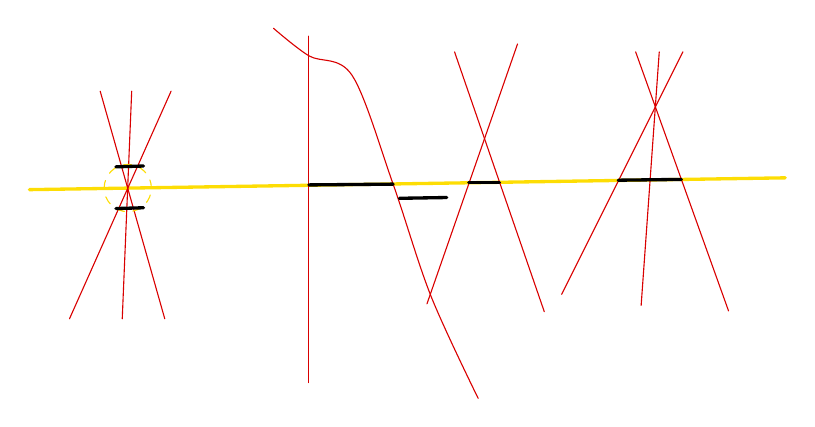
\begin{tikzpicture}[x=1mm,y=1mm,line cap=round,line join=round,font=\scriptsize]
\draw[Ye,very thick] (4,-26.5) -- (100,-25);
\draw[Rd] (13,-14) -- (21.2,-42.9);
\draw[Rd] (22,-14) -- (9.1,-42.9);
\draw[Rd] (17,-14) -- (15.8,-42.9);
\draw[Ye,dashed] (16.5,-26.3) circle[radius=3];
\draw[very thick] (15,-23.6) -- (18.5,-23.5);
\draw[very thick] (15,-28.9) -- (18.5,-28.8);
\draw[Rd] (39.5,-7) -- (39.5,-51);
\draw[Rd] plot[smooth, tension=0.55] coordinates {(35,-6) (39.5,-9.5) (45,-12) (50.2,-25.8) (55,-40) (61,-53)};
\draw[very thick] (39.5,-25.9) -- (50.2,-25.8);
\draw[Rd] (58,-9) -- (69.4,-42);
\draw[Rd] (66,-8) -- (54.5,-41);
\draw[very thick] (51,-27.6) -- (57,-27.5);
\draw[very thick] (59.8,-25.6) -- (63.7,-25.6);
\draw[Rd] (81,-9) -- (92.8,-41.9);
\draw[Rd] (87,-9) -- (71.6,-39.8);
\draw[Rd] (84,-9) -- (81.7,-41.2);
\draw[very thick] (78.8,-25.3) -- (86.8,-25.2);
\end{tikzpicture}
\end{document}
